%----------------------------------------------------------------------------
%
%	This template was created by
%		Christian Krieg <christian.krieg@alumni.tuwien.ac.at>
%
%	April 2018
%
%----------------------------------------------------------------------------
%
\documentclass[%
	a4paper,
]
{article}
%
%----------------------------------------------------------------------------
%
% Institution
%
%\institution{Institute of Computer Technology}
%
%----------------------------------------------------------------------------
%
% Use the 'Libertine' font type
%
\usepackage{libertine}
\usepackage[T1]{fontenc}
\usepackage[utf8]{inputenc}
%
%----------------------------------------------------------------------------
%
% Set page margins
%
\usepackage{geometry}
\geometry{%
	left   = 2cm,
	right  = 2cm,
	top    = 2cm,
	bottom = 2cm
}
%
%----------------------------------------------------------------------------
%
% Set line spacing
%
\usepackage{setspace}
\setstretch{1}
%
%----------------------------------------------------------------------------
%
% Set paragraph: No indentation, but include an empty line
%
\usepackage[parfill]{parskip}
%
%----------------------------------------------------------------------------
%
% Settings for hyperlinks
%
\usepackage{hyperref}
\hypersetup{%
	colorlinks = true,
	allcolors  = blue,
}
%
%----------------------------------------------------------------------------
%
% Use colors
%
\usepackage{xcolor}
\usepackage{colortbl}
%
%----------------------------------------------------------------------------
%
% Define a TODO and a DONE command
%
\newcommand{\todo}[1]{\textcolor{red}{#1}}
\newcommand{\done}[1]{}
%
%----------------------------------------------------------------------------
%
% Use glossaries
%
\usepackage{glossaries}
\makeglossaries
%
% Glossary entries
%
\newglossaryentry{fpga}{
	name = {FPGA},
	description = {Field-programmable gate array},
	text = {FPGA},
	first = {field-programmable gate array (FPGA)},
	plural = {FPGAs},
	firstplural = {field-programmable gate arrays (FPGAs)},
}
%
\newglossaryentry{trng}{
	name = {TRNG},
	description = {True-random number generator},
	text = {TRNG},
	first = {true-random number generator (TRNG)},
	plural = {TRNGs},
	firstplural = {true-random number generators (TRNGs)},
}
%
\newglossaryentry{bcd}{
  name={BCD},
  description={Binary-coded decimal},
  text={BCD},
  first={binary-coded decimal (BCD)},
}
%
\newglossaryentry{hdl}{
  name={HDL},
  description={Hardware description language},
  text={HDL},
  first={hardware description language (HDL)},
  plural={HDLs},
  firstplural={hardware description languages (HDLs)},
}
%
\newglossaryentry{ip}{
  name={IP},
  description={Intellectual property},
  text={IP},
  first={intellectual property (IP)},
}
%
\newglossaryentry{3pip}{
  name={3PIP},
  description={Third-party intellectual property},
  text={3PIP},
  first={third-party intellectual property (3PIP)},
}
%
\newglossaryentry{dsp}{
  name={DSP},
  description={Digital signal processor},
  text={DSP},
  first={digital signal processor (DSP)},
  plural={DSPs},
  firstplural={digital signal processors (DSPs)},
}
%
\newglossaryentry{amba}{
  name={AMBA},
  description={Advanced microcontroller bus architecture},
  text={AMBA},
  first={advanced microcontroller bus architecture (AMBA)},
}
%
\newglossaryentry{apb}{
  name={APB},
  description={Advanced peripheral bus},
  text={APB},
  first={advanced peripheral bus (APB)},
}
%
%\newglossaryentry{}{
%  name={},
%  description={},
%  text={},
%  first={},
%  plural={},
%  firstplural={},
%}
%
%----------------------------------------------------------------------------
%
% Using URLs
%
\usepackage{url}
%
%
%% Define a new style with a smaller font.
\makeatletter
\def\url@footnotestyle{%
  \@ifundefined{selectfont}{\def\UrlFont{\sf}}{\def\UrlFont{\footnotesize\rmfamily}}}
\makeatother
%% Now actually use the newly defined style.
\urlstyle{footnote}
%
%
%
%% Define a new style with a larger font.
\makeatletter
\def\url@normalstyle{%
  \@ifundefined{selectfont}{\def\UrlFont{\sf}}{\def\UrlFont{\normalsize\rmfamily}}}
\makeatother
%% Now actually use the newly defined style.
\urlstyle{footnote}
%
%----------------------------------------------------------------------------
%
% Settings for citations and the bibliography
%
\usepackage[%
	backend     = biber,
	maxbibnames = 99,
	autocite    = footnote,
	citestyle   = verbose-ibid,
	firstinits=true,
]{biblatex}
\bibliography{bib/stuff}
%
%----------------------------------------------------------------------------
%
%	TikZ -- TikZ ist kein Zeichenprogramm
%
\usepackage{tikz}
\usepackage{tikz-timing}
\usepackage{etoolbox}
\usetikzlibrary{mindmap}
\usetikzlibrary{shapes}
\usetikzlibrary{arrows}
\usetikzlibrary{decorations}
\usetikzlibrary{shapes.symbols}
\usetikzlibrary{shapes.geometric}
\usetikzlibrary{shapes.multipart}
\usetikzlibrary{positioning}
\usetikzlibrary{patterns}
\usetikzlibrary{calc}
\usetikzlibrary{scopes}         % cf. pgfmanual p.66
\usetikzlibrary{chains}         % cf. pgfmanual p.284
\usetikzlibrary{fit}
\usetikzlibrary{matrix}
\usetikzlibrary{decorations}
\usetikzlibrary{circuits.logic}
\usetikzlibrary{circuits.logic.IEC}
\usetikzlibrary{shapes.gates.logic.IEC}
\usetikzlibrary{circuits.logic.US}
\usetikzlibrary{shapes.gates.logic.US}
\usetikzlibrary{circuits.ee}
\usetikzlibrary{circuits.ee.IEC}
\usetikzlibrary{backgrounds}
\usetikzlibrary{automata}
\usetikzlibrary{intersections}
\usetikzlibrary{plotmarks}
\usepgflibrary{fpu}
\usetikzlibrary{decorations.pathreplacing}
%
%----------------------------------------------------------------------------
%
% TikZ shapes
%  
%	% D flip-flops (DFFs) and shift register
% Author: Martin Scharrer
%\documentclass[a4paper,landscape]{article}

%\usepackage{pgf,tikz}
%%%<
%\usepackage{verbatim}
%\usepackage[active,tightpage]{preview}
%\PreviewEnvironment{tikzpicture}
%\setlength\PreviewBorder{5pt}%
%%%>

%\begin{comment}
%:Title: D flip-flops and shift register
%
%Example of a custom node shape for drawing  D flip-flops. The shape is used to draw a serial shift
%register. 
%
%\end{comment}
%
%\usetikzlibrary{calc,arrows}
%\usepackage{amsmath}
%\usepackage[left=1cm,right=1cm]{geometry}
%\pagestyle{empty}

\makeatletter

% Data Flip Flip (DFF) shape
\pgfdeclareshape{dff}{
  % The 'minimum width' and 'minimum height' keys, not the content, determine
  % the size
  \savedanchor\northeast{%
    \pgfmathsetlength\pgf@x{\pgfshapeminwidth}%
    \pgfmathsetlength\pgf@y{\pgfshapeminheight}%
    \pgf@x=0.5\pgf@x
    \pgf@y=0.5\pgf@y
  }
  % This is redundant, but makes some things easier:
  \savedanchor\southwest{%
    \pgfmathsetlength\pgf@x{\pgfshapeminwidth}%
    \pgfmathsetlength\pgf@y{\pgfshapeminheight}%
    \pgf@x=-0.5\pgf@x
    \pgf@y=-0.5\pgf@y
  }
  % Inherit from rectangle
  \inheritanchorborder[from=rectangle]

  % Define same anchor a normal rectangle has
  \anchor{center}{\pgfpointorigin}
  \anchor{north}{\northeast \pgf@x=0pt}
  \anchor{east}{\northeast \pgf@y=0pt}
  \anchor{south}{\southwest \pgf@x=0pt}
  \anchor{west}{\southwest \pgf@y=0pt}
  \anchor{north east}{\northeast}
  \anchor{north west}{\northeast \pgf@x=-\pgf@x}
  \anchor{south west}{\southwest}
  \anchor{south east}{\southwest \pgf@x=-\pgf@x}
  \anchor{text}{
    \pgfpointorigin
    \advance\pgf@x by -.5\wd\pgfnodeparttextbox%
    \advance\pgf@y by -.5\ht\pgfnodeparttextbox%
    \advance\pgf@y by +.5\dp\pgfnodeparttextbox%
  }

  % Define anchors for signal ports
  \anchor{D}{
    \pgf@process{\northeast}%
    \pgf@x=-1\pgf@x%
    \pgf@y=.5\pgf@y%
  }
  \anchor{CLK}{
    \pgf@process{\northeast}%
    \pgf@x=-1\pgf@x%
    \pgf@y=-.66666\pgf@y%
  }
  \anchor{CE}{
    \pgf@process{\northeast}%
    \pgf@x=-1\pgf@x%
    \pgf@y=-0.33333\pgf@y%
  }
  \anchor{Q}{
    \pgf@process{\northeast}%
    \pgf@y=.5\pgf@y%
  }
  \anchor{Qn}{
    \pgf@process{\northeast}%
    \pgf@y=-.5\pgf@y%
  }
  \anchor{R}{
    \pgf@process{\northeast}%
    \pgf@x=0pt%
  }
  \anchor{S}{
    \pgf@process{\northeast}%
    \pgf@x=0pt%
    \pgf@y=-\pgf@y%
  }
  % Draw the rectangle box and the port labels
  \backgroundpath{
    % Rectangle box
    \pgfpathrectanglecorners{\southwest}{\northeast}
    % Angle (>) for clock input
    \pgf@anchor@dff@CLK
    \pgf@xa=\pgf@x \pgf@ya=\pgf@y
    \pgf@xb=\pgf@x \pgf@yb=\pgf@y
    \pgf@xc=\pgf@x \pgf@yc=\pgf@y
    \pgfmathsetlength\pgf@x{.75ex} % size depends on font size
    \advance\pgf@ya by \pgf@x
    \advance\pgf@xb by \pgf@x
    \advance\pgf@yc by -\pgf@x
    \pgfpathmoveto{\pgfpoint{\pgf@xa}{\pgf@ya}}
    \pgfpathlineto{\pgfpoint{\pgf@xb}{\pgf@yb}}
    \pgfpathlineto{\pgfpoint{\pgf@xc}{\pgf@yc}}
    \pgfclosepath

    % Draw port labels
    \begingroup
    \tikzset{flip flop/port labels} % Use font from this style
    \tikz@textfont

    \pgf@anchor@dff@D
    \pgftext[left,base,at={\pgfpoint{\pgf@x}{\pgf@y}},x=\pgfshapeinnerxsep]{\raisebox{-0.75ex}{D}}

%    \pgf@anchor@dff@CE
%    \pgftext[left,base,at={\pgfpoint{\pgf@x}{\pgf@y}},x=\pgfshapeinnerxsep]{\raisebox{-0.75ex}{CE}}

    \pgf@anchor@dff@Q
    \pgftext[right,base,at={\pgfpoint{\pgf@x}{\pgf@y}},x=-\pgfshapeinnerxsep]{\raisebox{-.75ex}{Q}}

%    \pgf@anchor@dff@Qn
%    \pgftext[right,base,at={\pgfpoint{\pgf@x}{\pgf@y}},x=-\pgfshapeinnerxsep]{\raisebox{-.75ex}{$\overline{\mbox{Q}}$}}
%
%    \pgf@anchor@dff@R
%    \pgftext[top,at={\pgfpoint{\pgf@x}{\pgf@y}},y=-\pgfshapeinnerysep]{R}
%
%    \pgf@anchor@dff@S
%    \pgftext[bottom,at={\pgfpoint{\pgf@x}{\pgf@y}},y=\pgfshapeinnerysep]{S}
    \endgroup
  }
}

% Key to add font macros to the current font
\tikzset{add font/.code={\expandafter\def\expandafter\tikz@textfont\expandafter{\tikz@textfont#1}}} 

% Define default style for this node
% \tikzset{flip flop/port labels/.style={font=\sffamily\scriptsize}}
%\tikzset{every dff node/.style={draw,minimum width=2cm,minimum 
%height=2.828427125cm,very thick,inner sep=1mm,outer sep=0pt,cap=round,add 
%font=\sffamily}}
\tikzset{flip flop/port labels/.style={font=\tiny}}
\tikzset{every dff node/.style={draw,minimum width=.75cm,minimum 
height=1cm,inner sep=1mm,outer sep=0pt,cap=round,font=\scriptsize}}

\makeatother

%\begin{document}
%
%\begin{tikzpicture}[font=\sffamily,>=triangle 45]
%  \def\N{7}  % Number of Flip-Flops minus one
%
%  % Place FFs
%  \foreach \m in {0,...,\N}
%    \node [shape=dff] (DFF\m) at ($ 3*(\m,0) $) {Bit \#\m};
%
%  % Connect FFs (Q1 with D1, etc.)
%  \def\p{0}  % Used to save the previous number
%  \foreach \m in {1,...,\N} { % Note that it starts with 1, not 0
%    \draw [->] (DFF\p.Q) -- (DFF\m.D);
%    \global\let\p\m
%  }
%
%  % Connect and label data in- and output port
%  \draw [<-] (DFF0.D) -- +(-1,0) node [anchor=east] {input} ;
%  \draw [->] (DFF\N.Q) -- +(1,0) node [anchor=west] {output};
%
%  % 'Reset' port label
%  \path (DFF0) +(-2cm,+2cm) coordinate (temp)
%    node [anchor=east] {reset};
%  % Connect resets
%  \foreach \m in {0,...,\N}
%    \draw [->] (temp) -| (DFF\m.R);
%
%  % 'Set' port label
%  \path (DFF0) +(-2cm,-2cm) coordinate (temp)
%    node [anchor=east] {set};
%  % Connect sets
%  \foreach \m in {0,...,\N}
%    \draw [->] (temp) -| (DFF\m.S);
%
%  % Clock port label
%  \path (DFF0) +(-2cm,-2.5cm) coordinate (temp)
%    node [anchor=east] {clock};
%  \foreach \m in {0,...,\N}
%    \draw [->] (temp) -| ($ (DFF\m.CLK) + (-5mm,0) $) --(DFF\m.CLK);
%
%  % Clock port label
%  \path (DFF0) +(-2cm,-3cm) coordinate (temp)
%    node [anchor=east] {clock enable};
%  \foreach \m in {0,...,\N}
%    \draw [->] (temp) -| ($ (DFF\m.CE) + (-7.5mm,0) $) --(DFF\m.CE);
%\end{tikzpicture}
%
%\end{document}

%
%----------------------------------------------------------------------------
%
% Use AMS math fonts
%
\usepackage{amsfonts}
\usepackage[sans]{dsfont}
%
%----------------------------------------------------------------------------
%
% Use multiple figures in one float
%
\usepackage{subcaption}
%
%----------------------------------------------------------------------------
%
% Use dummy text
%
\usepackage{lipsum}
%
%----------------------------------------------------------------------------
%
% Use extended list environments (e.g., 'inparaenum')
%
\usepackage{paralist}
%
%----------------------------------------------------------------------------
%
% Use listings
%
\usepackage{listings}

\lstdefinestyle{vhdl}
{
	language=VHDL,
  basicstyle=\linespread{1}\scriptsize\ttfamily\color{black},
  commentstyle=\scriptsize\itshape,
  escapeinside={(*@}{@*)},
  frame=single, numbers=left,
%  numbersep=5pt,
  xleftmargin=15pt,
  xrightmargin=5pt,
  numbersep=5pt,
  breaklines=true,
  moredelim=**[is][\ttfamily\bfseries\color{red}]{(*}{*)},
}

\lstdefinestyle{verilog}
{
	language=Verilog,
  basicstyle=\linespread{1}\scriptsize\ttfamily\color{black},
  commentstyle=\scriptsize\itshape,
  escapeinside={(*@}{@*)},
  frame=single, numbers=left,
%  numbersep=5pt,
  xleftmargin=15pt,
  xrightmargin=5pt,
  numbersep=5pt,
  breaklines=true,
  moredelim=**[is][\ttfamily\bfseries\color{red}]{(*}{*)},
}
%
%----------------------------------------------------------------------------
%
% Typeset pseudo code
%
\usepackage{syntax}
%
%----------------------------------------------------------------------------
%
% More options for boxes
%
\usepackage{realboxes}
%
% Command for vertical text in tabulars
%
\newcommand*\rot{\rotatebox{90}}
%
%----------------------------------------------------------------------------
%
% Use \textsubscript
%
\usepackage{fixltx2e}
%
%----------------------------------------------------------------------------
%
% More options for tabulars
%
\usepackage{array}
%
%----------------------------------------------------------------------------
%
% Use appendices
%
\usepackage[titletoc]{appendix}
%
%----------------------------------------------------------------------------
%
% Use the cleverref package -- Load this package as the very last!
%
\usepackage{cleveref}


\usepackage{import}
\usepackage{xifthen}
\usepackage{pdfpages}
\usepackage{transparent}

\newcommand{\incfig}[2]{%
    \def\svgscale{#2}
    \import{./fig/}{#1.pdf_tex}
}


\newcommand{\DrawData}[5]{
        \draw plot [mark=#1, mark size=25,  mark options={#2}] coordinates{( #3 , #4 , #5 )}; 
        \draw[very thin,gray] ( #3 , 0 , #5 ) -- ( #3 , #4 , #5 ) node[right] { (#3 #4 #5)} ;
        \draw[very thin,gray] ( #3 , 0 , #5 ) -- ( #3 , 0 , 0 ) ;
        \draw[very thin,gray] ( #3 , 0 , #5 ) -- ( 0 , 0 , #5 ) ;
}
\newcommand{\DrawDataUnmarked}[5]{
        \draw plot [mark=#1, mark size=25,  mark options={#2}] coordinates{( #3 , #4 , #5 )}; 
        \draw[very thin,gray] ( #3 , 0 , #5 ) -- ( #3 , #4 , #5 ) ;
        \draw[very thin,gray] ( #3 , 0 , #5 ) -- ( #3 , 0 , 0 ) ;
        \draw[very thin,gray] ( #3 , 0 , #5 ) -- ( 0 , 0 , #5 ) ;
}



\usepackage{float}
\usepackage{graphicx}
\usepackage{rotating}
\usepackage{pdflscape}
%
%----------------------------------------------------------------------------
%
% Document body
%
\begin{document}
\newcommand{\Hilight}{\makebox[0pt][l]{\color{yellow}\rule[0pt]{\linewidth}{5pt}}}

%
%----------------------------------------------------------------------------
%
\begin{titlepage}

	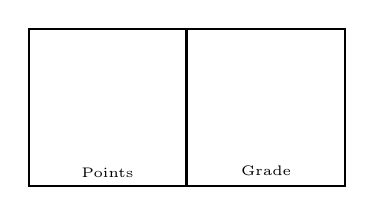
\begin{tikzpicture}[thick]
		\node (points) at (0,0) [draw,minimum size=2cm] {};
		\node (lbl-points) at (points.south) [anchor=south,font=\tiny] {Points};
		\node (grade) at (points.east) [draw,minimum size=2cm,anchor=west,
			outer sep=0] {};
		\node (lbl-grade) at (grade.south) [anchor=south,font=\tiny] {Grade};
	\end{tikzpicture}

	\begin{flushright}

		% Update this with your team number
		\huge\bfseries
		Team: XX \\[1em]

		% Update this with your matriculation number, first name, second name
		\large
		1525864 Andreas Glinserer	\\
	
	\end{flushright}

	\vspace{5em}

	\begin{center}
		{\huge Digital Integrated Circuits Lab (LDIS)}\\[1em]
		{\Large 384.088, Summer Term 2019} \\[2em]
		{\large Supervisors:\\[.5em]
			Christian Krieg, David Radakovits, Axel Jantsch} \\[10em]

		{\Huge Task 3:\\[.5em]AMBA Digital Thermometer,\\[.5em] Design Documentation}\\[10em]
	\end{center}


%	\begin{abstract}
%
%		Enter the abstract of your report here. An abstract summarizes your
%		entire work (i.e., problem statement, motivation, methodology, key
%		findings). It is a good strategy to write a first version of the abstract
%		when you start to work on your report. This gives you a good guideline
%		what to	put and what not to put into the report. Ideally, you re-write
%		the abstract once you finished your report, because only at this point
%		you have all the information available to create a good abstract.
%
%	\end{abstract}

\end{titlepage}
%
%----------------------------------------------------------------------------
%
\tableofcontents

\section{Digital Thermometer with AMBA}
\label{sec:characterization}

This design is used to instantiate a digital thermometer on the Nexys4 DDR.
A possible instantiation of the design can be seen in \textbf{./src/AMBA_digitherm.vhd}.


The digital thermometer consists of 5 indepent parts which work together:
\begin{description}
\item[AMBA APB Master] - This part controls the whole design and calls 
the other parts according to the wanted way operation. It consists of 
two state machines where both consist of two processes. This part lies within
the \mbox{\textbf{./src/AMBA_CTL.vhd}} file.
\item[Data Sampling] - This part configures the temperature sensor, which 
is an \autocite{ADT7420}, and requests the data in a regular interval. This interval 
is fixed in the design and is set to 1 second. This part lies within the 
\mbox{\textbf{./src/AMBA_Slave_ADT.vhd}} file.
\item[Data Processing] - The thermometer uses a moving average filter
to mitigate sudden jumps in the data. The filter width is variable and
is controlled by another part of the design. This part lies within the 
\mbox{\textbf{./src/AMBA_Slave_DSP.vhd}} file.
\item[Data Output] - The processed data gets calculated here by using the 
double dabble algorithm\footnote{Sites for Explanation: Wikipedia: \url{https://en.wikipedia.org/wiki/Double_dabble}, Youtube: \url{https://www.youtube.com/watch?v=eXIfZ1yKFlA}}. Apart from that
it manages the multiplexing of the seven-segment display. This part lies 
within the \mbox{\textbf{./src/AMBA_Slave_Output.vhd}} file.
\item[Switch Polling] - Polls the switch regularly to get the current switch
state. If the state differs (the size of the moving average changed) it starts
an extra cycle to tell the Data Processing to restart with a new window size.
This part lies within the \mbox{\textbf{./src/AMBA_Slave_Switch}} file.
\end{description}

Each of the mentioned parts (except the Switch Polling) above instantiates the real part and an apb\autocite{apb}-interface
for the bus communication. Each of these standalone parts get explained in the next 
section in detail. Within Fig.\ref{fig:system} you can see a schematic overview of the system
and how the parts are all connected via the apb-interface.

\begin{figure}[H]
		\centering
		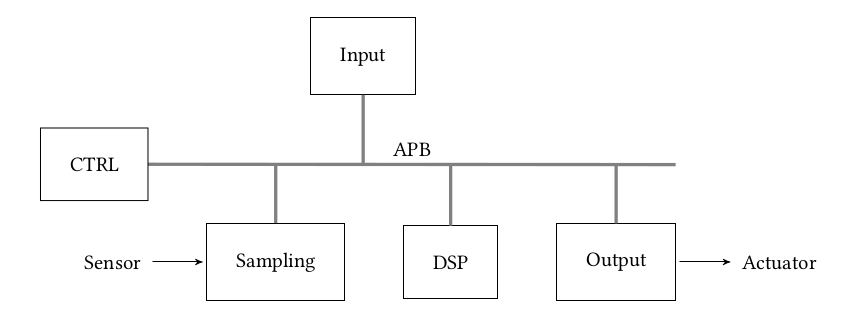
\includegraphics[width=0.8\linewidth]{fig/system}
		\caption{Overview of the digital thermometer system. Source: Task 2 Description}
		\label{fig:system}
\end{figure}


\section {Implementation}
In this section i explain in more detail how everything is implemented. This design uses
 an active low reset for this task, which is the onboard switch with the name SW15.

\subsection{Sampling}
The sampling part of the design lies within the file \textbf{./src/ADT7420-Sampler.vhd} 
and instantiates the i2c-interface within \textbf{./src/TWICtl.vhd}.
\textbf{These two files were taken from the Nexys-4-OOB demo.}
For the reading of the temperature the onboard I2C-sensor is used. To get the values the
 the IP-core from the \autocite{Nexys-4-OOB} Demo which includes an readout of this sensor
 is used.
The sensor itself is an ADT7420 I2C temperature sensor. 
The output of the sampling part is:
\begin{description}
\item[out\_vld] - 1bit. It signals that a new value was read. It is high for one clock cycle after a 
successful read from the sensor.
\item[out\_data] - 16bit. The read temperature value gets output here. It holds the value and does
only change on the rising edge of the out\_vld.
\end{description}
Furthermore it toggles the LED4 everytime it retrieves a value.

\subsubsection{Changes to TWICTL.vhd}
The TWI Controller file was changed only in the way to use the ieee.numeric\_std.all library and 
all occurences which led to the errors with the new library.
Other than that this file is original.

\subsubsection{Changes to ADT7420-Sampler.vhd}
To the sampler were made some changes to get the wished functionality.
To get 16 bit readouts I added another init vector:

\lstset{style=vhdl, firstnumber=118}
\begin{lstlisting}
(*@\Hilight@*)constant NO_OF_INIT_VECTORS : natural := 4; -- number of init vectors in TempSensInitMap
constant DATA_WIDTH : integer := 1 + 8 + 8; -- RD/WR bit + 1 byte register address + 1 byte data
constant ADDR_WIDTH : natural := natural(ceil(log(real(NO_OF_INIT_VECTORS), 2.0)));

type TempSensInitMap_type is 
	array (0 to NO_OF_INIT_VECTORS-1) of std_logic_vector(DATA_WIDTH-1 downto 0);
signal TempSensInitMap: TempSensInitMap_type := (
IRD & x"0B" & x"CB", -- Read ID R[0x0B]=0xCB
IWR & x"2F" & x"00", -- Reset R[0x2F]=don't care
IRD & x"0B" & x"CB", -- Read ID R[0x0B]=0xCB
(*@\Hilight@*)IWR & x"03" & x"80"  -- configure it for 16bit
);
\end{lstlisting}

To get the sampling timing right i added an extra state in which the I2C waits.

\lstset{style=vhdl, firstnumber=101}
\begin{lstlisting}
constant SAMPLECNT : NATURAL := natural(ceil(real(clockfreq*1_000_000/Samples)))*2;

-- State Machine states definition
type state_type is (
	stIdle, -- Idle State
	stInitReg,  -- Send register address from the init vector
	stInitData, -- Send data byte from the init vector
	stRetry,    -- Retry state reached when there is a bus error, will retry RETRY_COUNT times
	stReadTempR,  -- Send temperature register address
	stReadTempD1, -- Read temperature MSB
	stReadTempD2, -- Read temperature LSB
	stError, -- Error state when reached when there is a bus error after a successful init; stays here until reset
(*@\Hilight@*)        stWait  -- State to wait for the next sample
);
signal state, nstate : state_type;
\end{lstlisting}

The new state was also added to the ReadyFlag process. This is needed to get the toggling right.

\lstset{style=vhdl, firstnumber=252,caption={Ready flag process. Here an error was encountered which is discussed in section \ref{problems}},label={lst:rdy-flag}}
\begin{lstlisting}
----------------------------------------------------------------------------------
-- Ready Flag
----------------------------------------------------------------------------------  
ReadyFlag: process (in_clk)
begin
	if Rising_Edge(in_clk) then
(*@\Hilight@*)		if (state = stIdle or state = stError) or state = stWait then
			fReady <= false;
		elsif (state = stReadTempD2 and twiDone = '1' and twiErr = '0') then
			fReady <= true;
		end if;
	end if;
end process;
\end{lstlisting}

In the OUTPUT\_DECODE process another when statement got added.
\lstset{style=vhdl, firstnumber=349, caption={}, label={lst:out-dec}}
\begin{lstlisting}
(*@\Hilight@*)when stWait =>
(*@\Hilight@*)	null;
\end{lstlisting}

In the NEXT\_STATE\_DECODE process the stReadTempD2 state got changed and another state got added:
\lstset{style=vhdl, firstnumber=410, label={lst:new-sta-dec}}
\begin{lstlisting}
when stReadTempD2 =>
	if (twiDone = '1') then
		if (twiErr = '1') then
			nstate <= stError;
		else
(*@\Hilight@*)			nstate <= stWait;
(*@\Hilight@*)--                  nstate <= stReadTempR; -- old version
		end if;
	end if;
 
(*@\Hilight@*)when stWait =>
(*@\Hilight@*)	if waitSample = SAMPLECNT then
(*@\Hilight@*)		nstate <= stReadTempR;
(*@\Hilight@*)	end if;
\end{lstlisting}

And a whole new process got added in which the counting happens for the sampling rate:
\lstset{style=vhdl, firstnumber=265, label={lst:smp-cnt}}
\begin{lstlisting}
---------------------------------------------------------------------------------- 
-- Sample counter wait               
----------------------------------------------------------------------------------  
SAMPLEWAIT : process(in_clk)                                       
begin                                                       
	if rising_edge(in_clk) then   
		if state = stWait then                       
			if waitSample = SAMPLECNT then             
				out_led <= led_helper; 
				led_helper <= not led_helper; 
			else 
				waitSample <= waitSample+1; 
			end if;                                                            

		else                                                                   
			waitSample <= 0;
		end if;                  
	end if;                 
end process;
\end{lstlisting}

\subsection{DSP}
\label{sec:dsp}

The moving average filter lies within the file \textbf{./src/DSP.vhd}.
The moving average is implemented as a state machine. The size of the filter window is determined
by the 3 switches SW2, SW1 and SW0. With these 3 switches you determine the binary number which 
then is used as the power for 2 for the filter size. So SW0 equals 1, SW1=2 and SW2=4.


Short example for this:
If SW2 is switched on and the others off, then the size equals $2^{4}=16$. \\Or if SW0 and SW1 are both on then the
size equals $2^{2+1}=8$. 


It is done this way to make the divison for the mean value easier, since
divison by a number which is a power of two equals a bitshift to the right.
The formula of the mean averge is dependent on the size $n$ which gets choosen by the switches.

A short description of the relevant ports:
\begin{description}
\item[in\_drdy] A rising edge on this signals a new value which should be put into the DSP.
\item[in\_data] The actual data which should be averaged as an 16 bit wide vector.
\item[in\_size] The power of two size binary encoded as explained earlier in a vector of width 3.
\item[out\_vld] This pin is high when the value at out\_avg is valid.
\item[out\_avg] The averaged data is output on this 16 bit wide vector.
\end{description}


\begin{equation*}
y = \sum_{i=0}^n x[i],
\end{equation*}
where $n$ equals the filter length and $i=0$ represents the most recent value in the buffer. This way the mean average is causal but the mean
value is shifted if you print it against the original values.


When the size gets changed the buffer gets set to zero. It then gets slowly refilled and the temperature
which gets sent to the BCD slowly increases, because it uses the fixed size for the division. 
It is done this way to show the working of the filter on the FPGA.

\subsection{Output}
The output part lies within the file \textbf{./src/7seg.vhd}
The output part gets the averaged temperature from the APB Master (or to be precise from the APB slave interface).
The hard part is to get from the binary value to a 
representation which fits on the BCD. One cannot just take the usual 4 bit approach for a segment 
because in the decimal system values only range from 0 to 9. So if the value would be an B in hex
one needs to subtract from the current position and add to the next position. This problem is solved
by using the double dabble algorithm.

Since the BCD share the anode contact there is also the need to multiplex the data which gets
to the corresponding outputs. This is done with the out\_an outputs. It is also important to notice
that the active selected anode is active low.

This is solved in two processes. The first process takes the data in if the valid flag is high. Contrary to 
DSP part it calculates the double dabble with for loops instead of a state machine. It then saves its
solutions to variables. The second process takes these solutions, converts it to an integer format and
uses these as indices for a predefined map of outputs. Furthermore the second process does this about
800 times per second to get a refresh rate of $100~\text{Hz}$ per BCD. This is done with a simple counter signal.

The ports explained:
\begin{description}
\item[in\_vld] Signals if the data is valid. New values are only calculated if this bit is high.
\item[in\_tmp] The value which shall be displayed on the BCD. 16 Bit Vector.
\item[out\_seg] The value for the selected BCD segment. 8 Bit Vector with active low values.
\item[out\_an] The selected anode which should be displayed. 8 Bit Vector where the selected segments
are active low.
\end{description}


\subsection{Master CTRL}
The master is implemented via 2 state machines. 
Every state machine is implemented with 2 processes. 1 process
which handles the outputs and another process which handles
the evaluation of the next state. The state change happens in
a synchronous process.
1 of the state
machines handles the APB Protocol and Data exchange on the line. 
It is built after the state machine (fig.\ref{fig:apb-state}) in the AMBA protocol pdf.

\begin{figure}[ht]
    \centering
    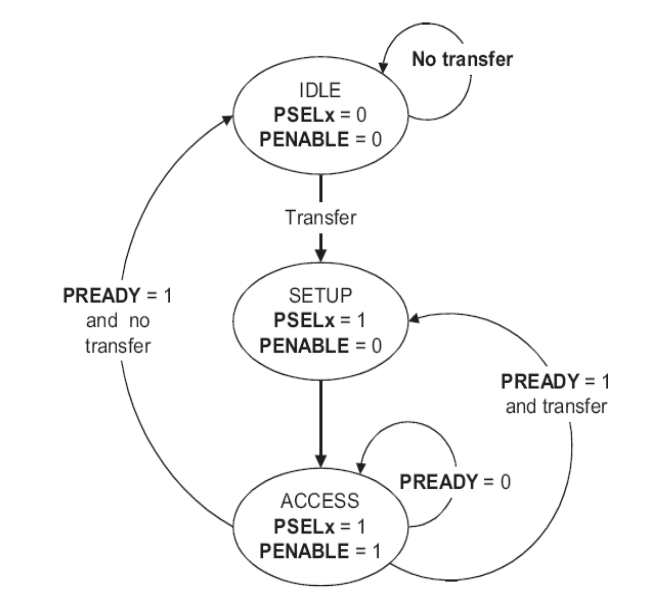
\includegraphics[scale=0.3]{fig/apb-state-diag.png}
    \caption{APB state diagram. Source:\protect\autocite{apb}}
    \label{fig:apb-state}
\end{figure}

The second state machine handles the program procedure (fig.\ref{fig:mst-state}). The 
procedure is as follows: Every $100\,\text{ms}$ it checks if
the switches changed. If a change happened then the new size
gets transmitted to the DSP. Every 
$\dfrac{1}{\text{samples}}\,\text{s}$ it reads the
Sampling part, writes this data then to the DSP, reads the DSP
and then transmits the output from the DSP to the output all over the APB interface.

\begin{figure}[ht]
    \centering
    \incfig{master-state-diagram}{1.7}
    \caption{master state diagram. Source: Drawn in Inkscape}
    \label{fig:mst-state}
\end{figure}

The master only utilizes the APB interface, therefore is no further
explanation of the different ports.

\subsection{APB slaves}
The slaves were implemented with the goal to leave the working
parts untouched. This goal was reached by implementing the
slaves as registers. The master writes to the registers and
the slave component reads from the register. Essentially every
slave consists of one read register to put the data on the bus 
and one write register to get the data from the bus. The naming
happened from the masters point of view, that is the reason for the
little naming contradiction (reading from the write register and 
writing to the read register).
Therefore every slave looks the same with slight modifications:

\lstset{style=vhdl, caption={ADT-Slave Template}, label={lst:apb-slv-tmp}}
\begin{lstlisting}
enable_write <= in_PENABLE and in_PWRITE and in_PSELx;
enable_read  <= not in_PWRITE and in_PSELx;     -- data is read everytime to be ready on the first cycle

out_PREADY <= int_pready;

-- register with the enable sigs as clock
WRITE: process(in_PRESETn, enable_write)
begin
        if in_PRESETn ='1' then
                int_data_write <= x"0000";

        elsif rising_edge(enable_write) then
                int_data_write <= in_PWDATA;
        end if;
end process WRITE;

-- register with the enable sigs as clock
READ: process(in_PRESETn, enable_read)
begin
        if in_PRESETn ='1' then
                out_PRDATA <= x"0000";

        elsif rising_edge(enable_read) then
                out_PRDATA <= int_data_read;

        end if;
end process WRITE;

PREADYP: process(enable_write, enable_read)
begin
        if enable_write='1' or enable_read='1' then
                int_PREADY <= '1';
        else
                int_PREADY <= '0';
        end if;
end process PREADYP;

-- process to forward the data to whatever module or to write into the read register
SFORWARD: process(in_PRESETn, in_PCLK, enable_write, in_PADDR)
begin

        if rising_edge(in_PCLK) then
                if in_PRESETn = '0' then
                        int_data_read <= x"0000";
                else
                        -- here comes handling of signals to write into the read register

                end if; -- rst
        end if; -- rising clock
end process SFORWARD;
\end{lstlisting}

For every slave a new .vhd file was created with the sceleton-template 
(see Listing \ref{lst:apb-slv-tmp}) above in it and an 
instantiation of the component it is the interface to. The ADT slave samples values
and if the CTRL requests values faster it just gets the old value back. If you write
to the DSP part, and want to read the new DSP value it holds the bus transmission by 
holding the PREADY signal low until the new value is computed.



\section{Simulation}
In this section the different simulations results are included and a short description for
everyone.

\begin{description}


\item[\hyperlink{sim1.1}{Simulation 1}] In this simulation you can see how the Master requests the Switches more often than he does
with the other parts. This is visible by looking at the in\_pready line. The short sequences are
those where the switch is polled and the longer are those where the the new value gets polled,
and sent to the DSP and the output.

\item[\hyperlink{sim2.1}{Simulation 2}] In this simulation you see a closer look of one normal transmission. The master
selects each of the slaves one after another with the out\_pselx respectively the slaves with each 
of his own in\_pselx wires. And you can also see that a transmission ends with the pready signal. 
Furthermore you can see that the DSP takes up multiple cycle when you read immediately after you
write. This is because the DSP blocks the transmission until a new value is computed.

\item[\hyperlink{sim3.1}{Simulation 3}] In this simulation you can see the calculation of a new value in the 
DSP part. With a given buffer size of 4 it takes up 4 calculations to reach the input value.

\item[\hyperlink{sim4.1}{Simulation 4}] In this simulation you can see the multiplexing of the bcd outputs. This
is visible in the the lines dbg\_an which selects the corresponding anode for one BCD and 
dbg\_seg which is the data that should be shown on the output.
\end{description}
\newpage

%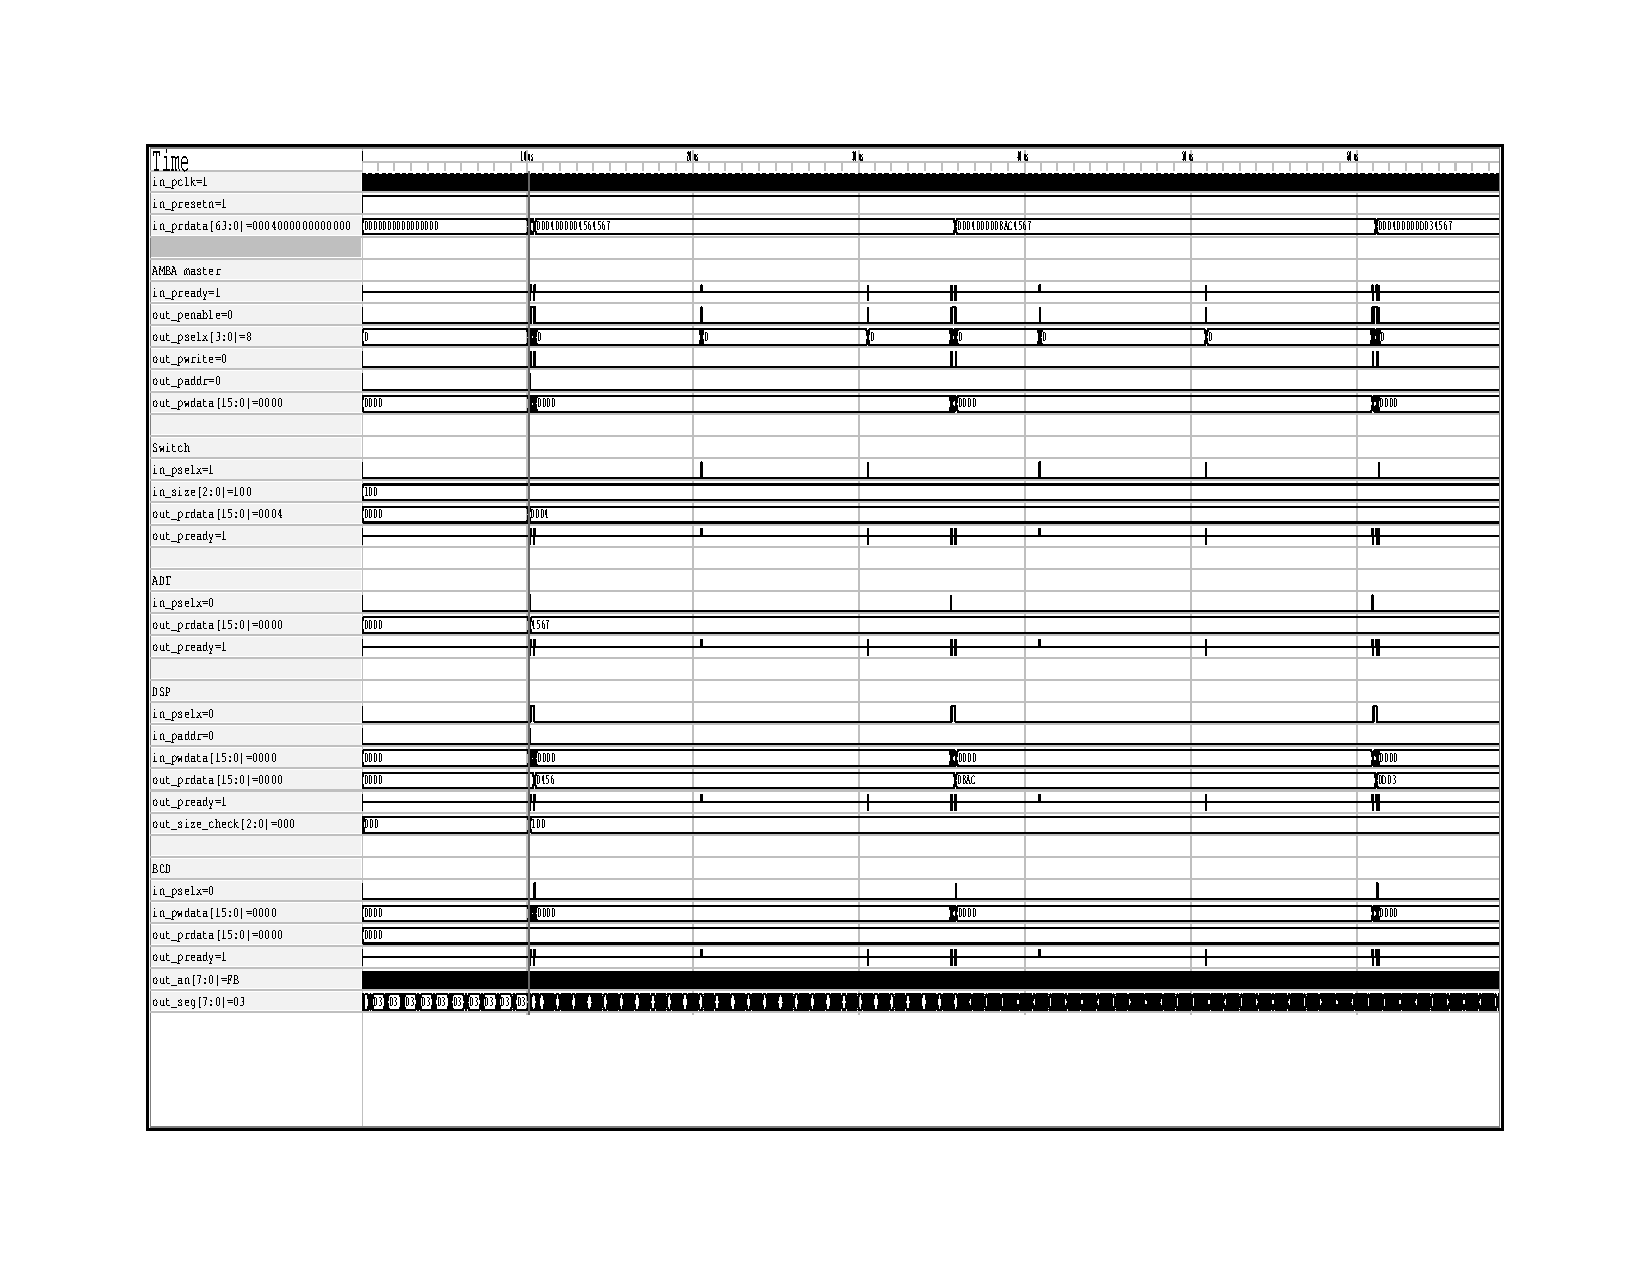
\includegraphics[angle=90]{./fig/simulation1.pdf}

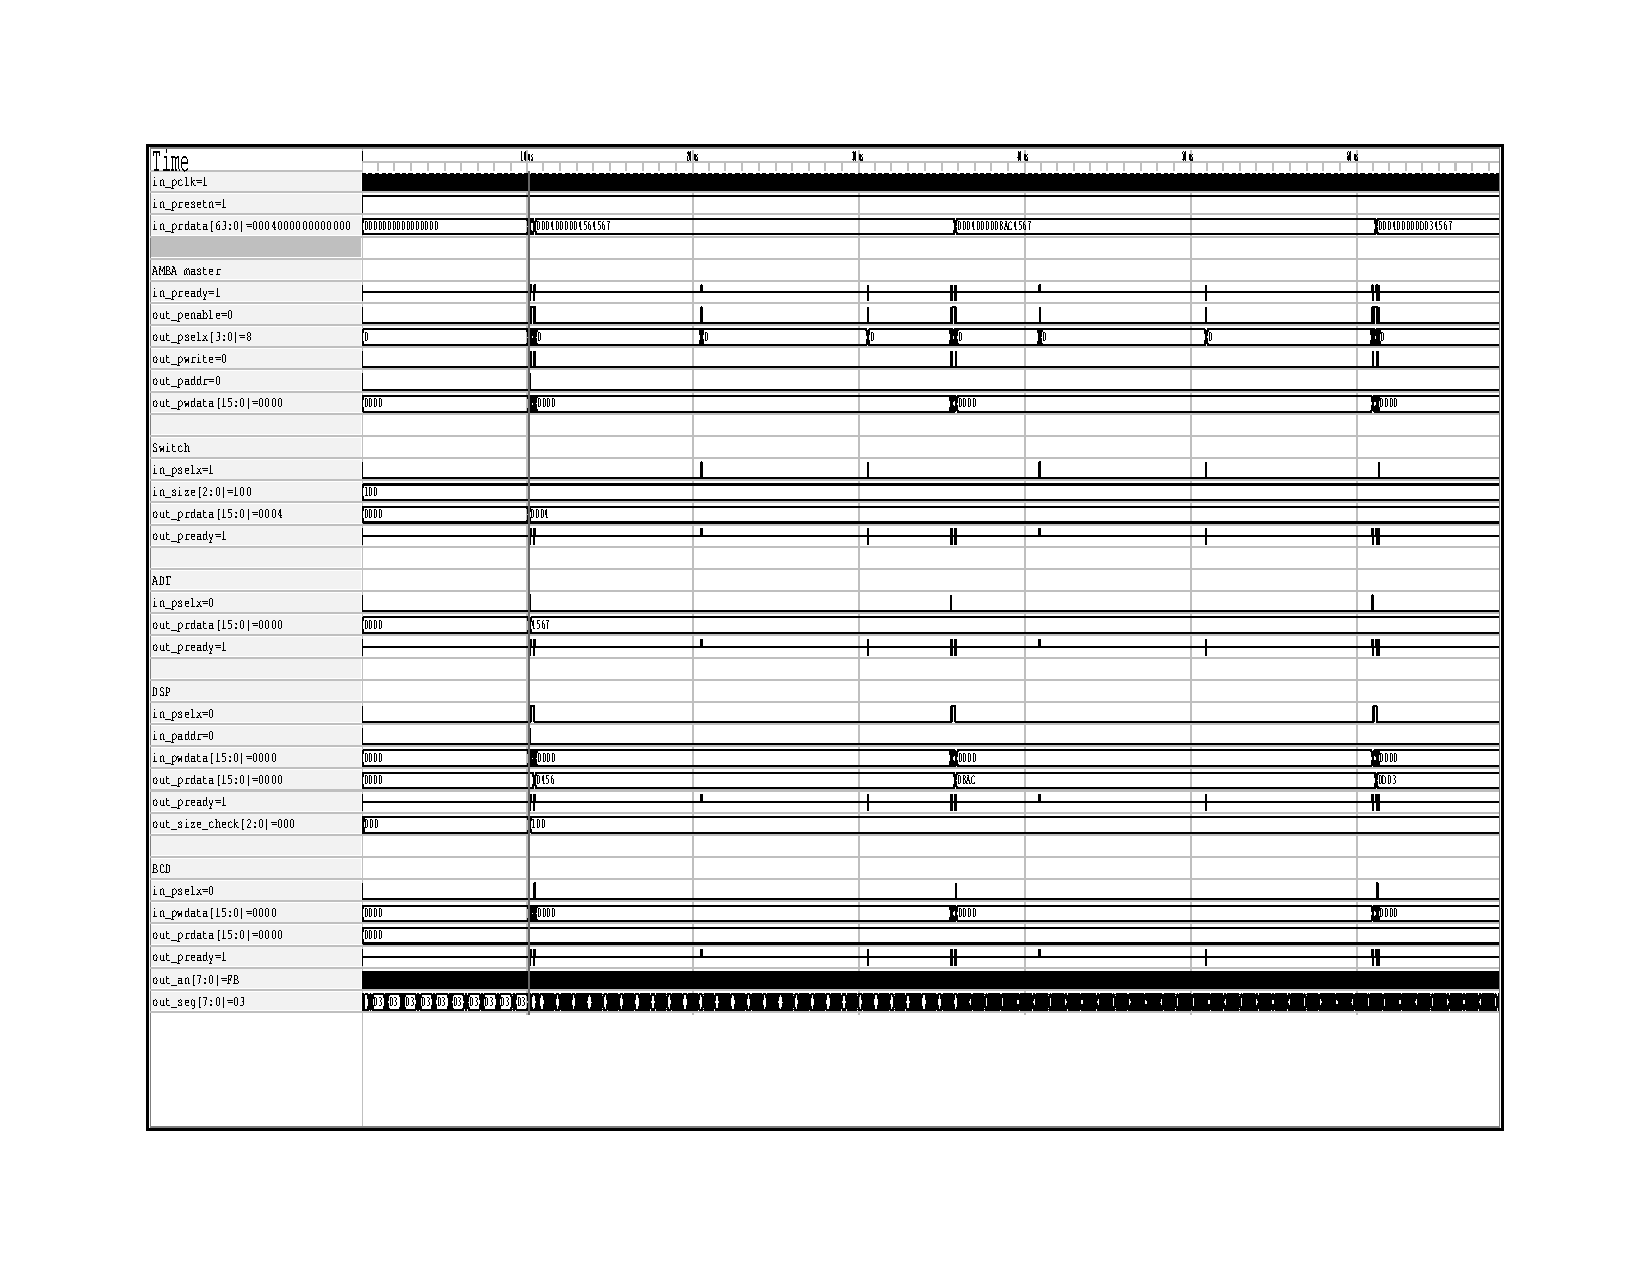
\includepdf[landscape=true,pages=1,scale=.9,link,linkname=sim1,pagecommand={},picturecommand*={\put (\LenToUnit{.05\paperwidth},20) 
{Simulation 1 to see the working master toggle the switches.}
;}]{./fig/simulation1.pdf}


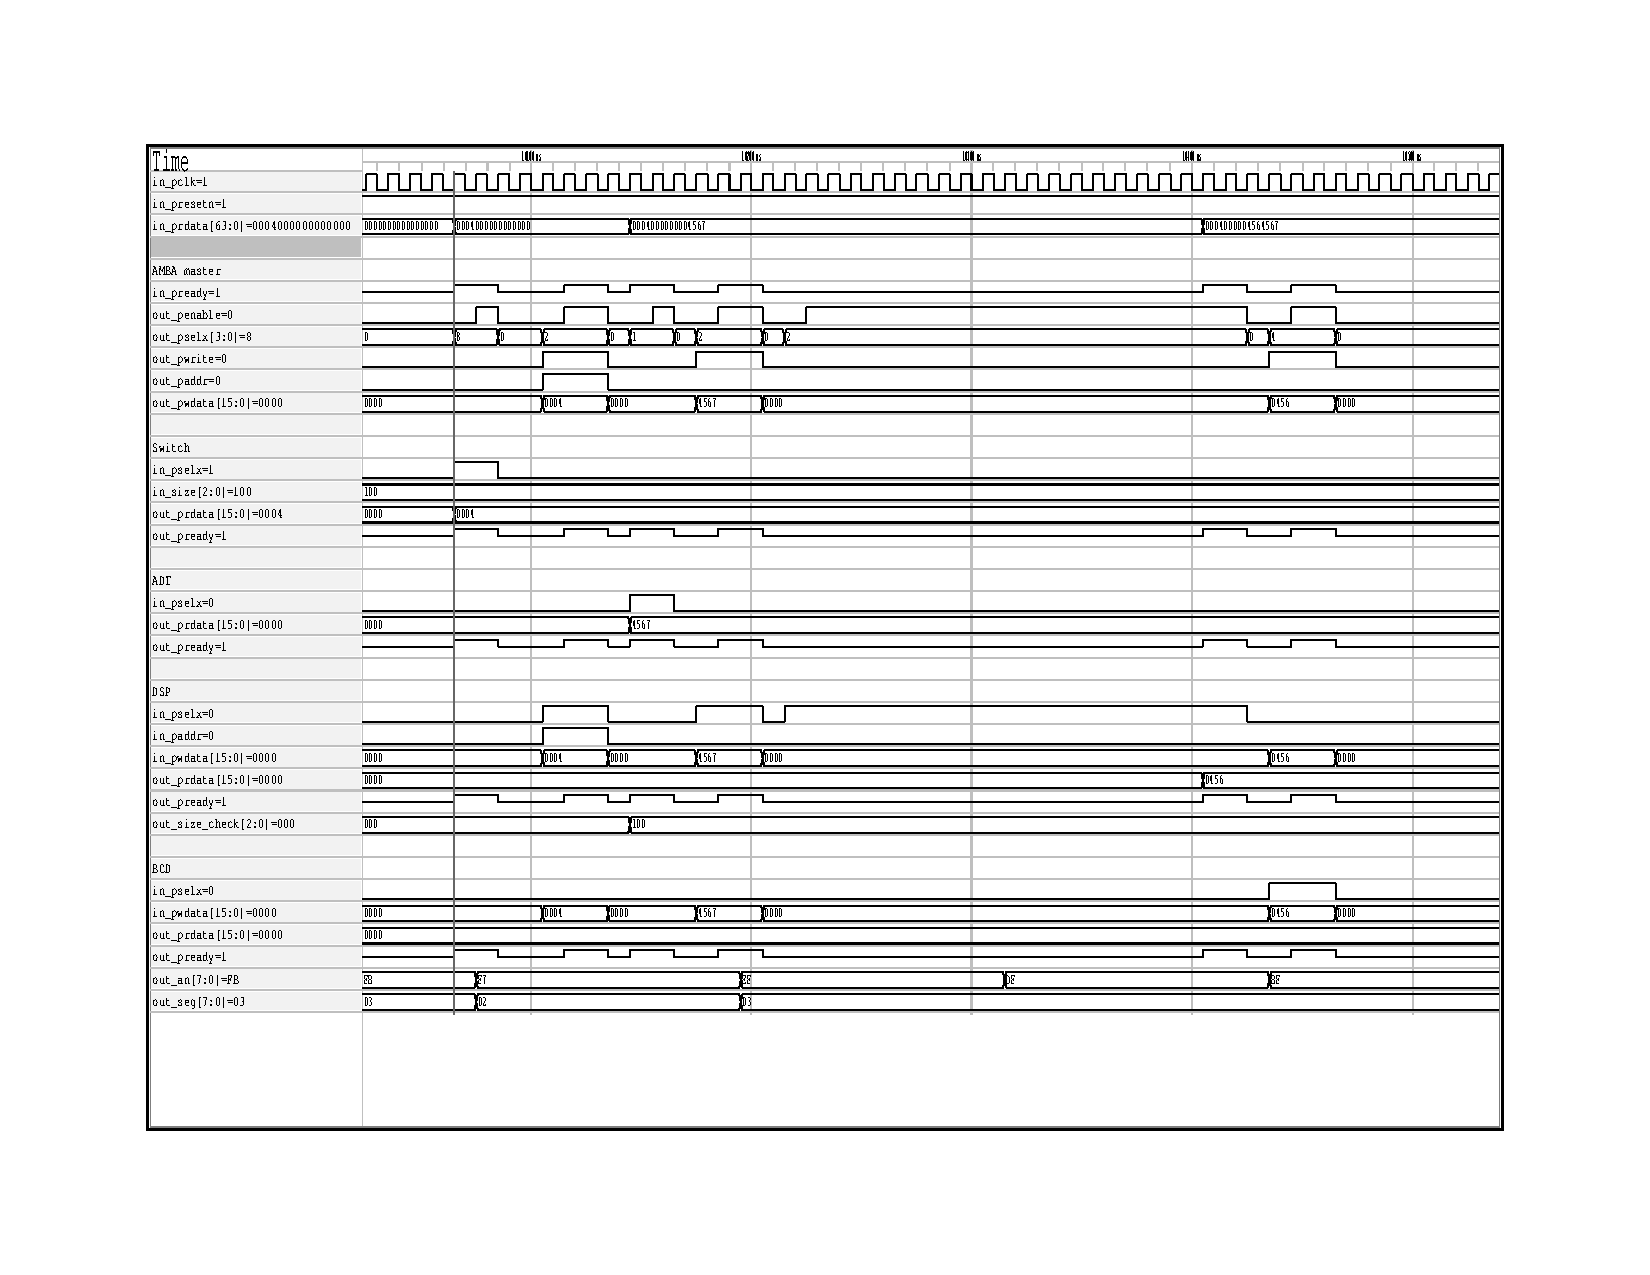
\includepdf[landscape=true,pages=1,scale=.9,pagecommand={},picturecommand*={\put (\LenToUnit{.05\paperwidth},20) 
{Simulation 2 which shows one transmission close up.}
;},link,linkname=sim2]{./fig/simulation2.pdf}


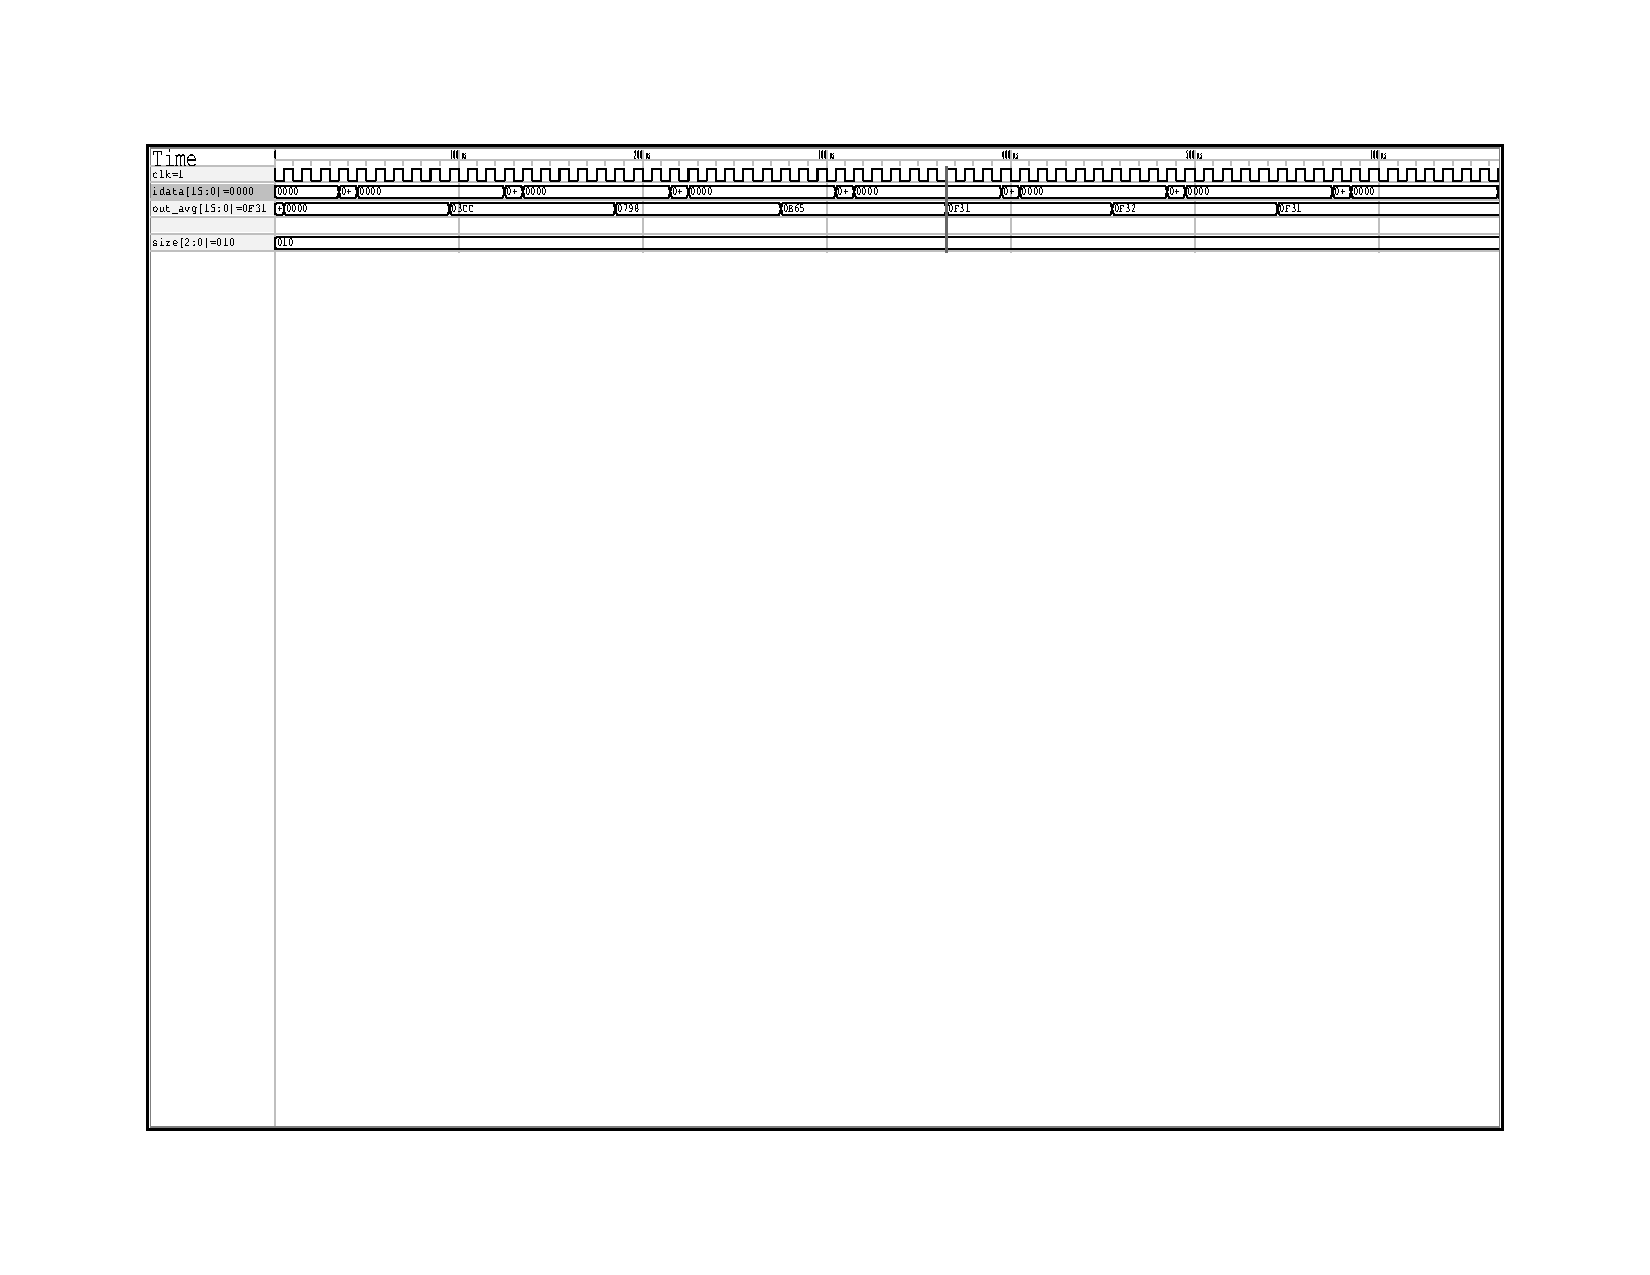
\includepdf[landscape=true,pages=1,scale=.9,pagecommand={},picturecommand*={\put (\LenToUnit{.05\paperwidth},20) 
{Simulation 3 which shows the DSP.}
;},link,linkname=sim3]{./fig/dsp-sim.pdf}

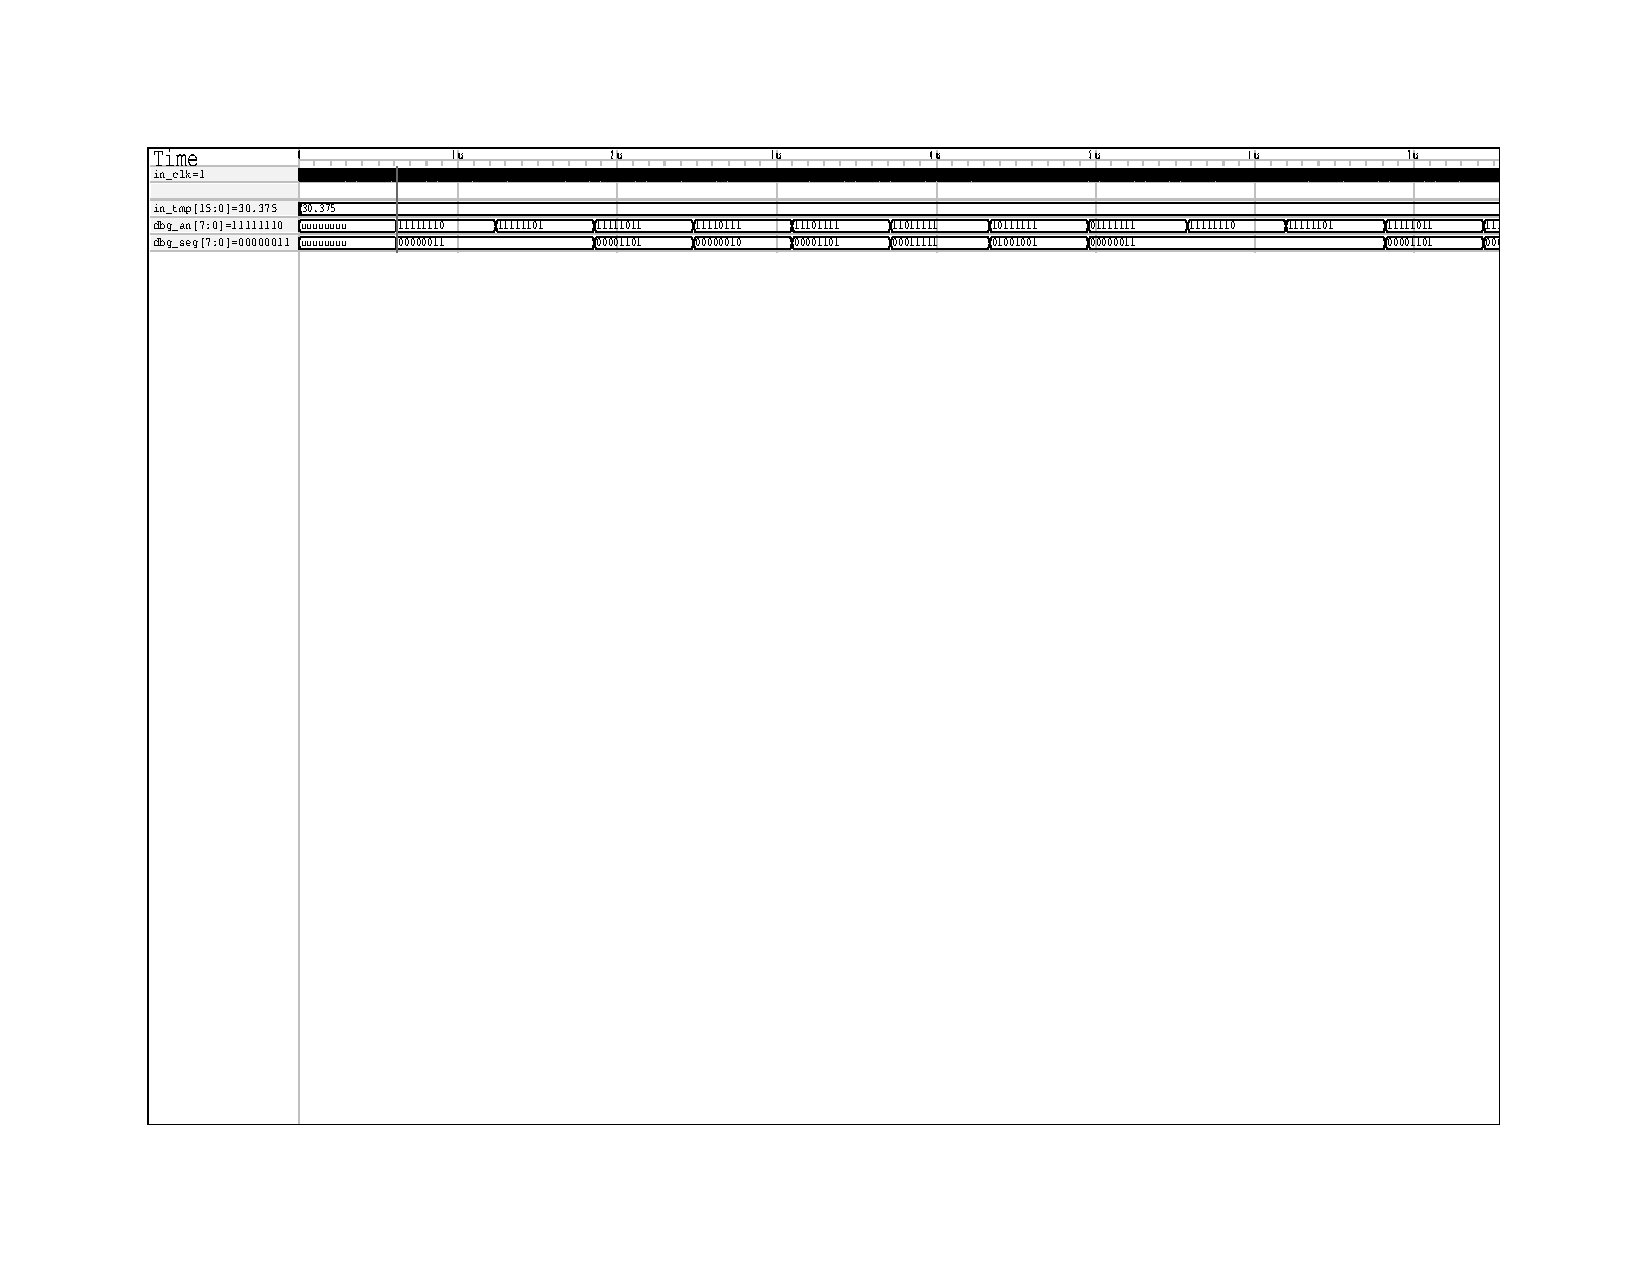
\includepdf[landscape=true,pages=1,scale=.9,pagecommand={},picturecommand*={\put (\LenToUnit{.05\paperwidth},20) 
{Simulation 4 which shows the multiplexing of the output.}
;},link,linkname=sim4]{./fig/sevseg-sim.pdf}




\section{Characterization}
Part of the lab was to characterize your design and compare it to other designs. Within 
table \ref{tab:characterization} are the values which were used for the comparision. This 
design corresponds to the entry of \textbf{Glinserer Andreas}. Furthermore a visualization
of the table can be seen within Fig. \ref{fig:characterization}. The other designs are 
marked with an 'X' and this design with an 'O'. 
\begin{table}[ht]
    \centering
    \begin{tabular}{l|lll}
         Group & $\text{t}_\text{{max}} [\text{ns}]	$ & $\text{P}_\text{avg} [\text{mW}]$ & $\text{r} [\%] $ \\ \hline \hline
        Philipp, Benedikt &	5,44	& 88,00	& 6,60 \\
        Kratzmann &	5,03 &	185,00 & 13,12 \\
        Essbüchl Jakob &	37,62 &	140	& 1,36 \\
        Glinserer Andreas &	5,89 &	110	& 1,54 \\ 
        Hauk Raphael &	8,08 &	111 &	3,9 \\
        Philipp W. &	2,557 &	121 &	0,477\\
        \hline
    \end{tabular}
    \caption{table with the design characterization from the other groups}
    \label{tab:characterization}
\end{table}
The value is calculated by summing up the used values in the utilization report
(section 1. Slice Logic)
and dividing them
by the summed up available values. The relevant snippet from the report can be seen
in Lst. \ref{lst:utilzation}.

\begin{lstlisting}[caption=Relevant part from the report\_utilization command needed for calculating the hardware utilization.,firstnumber=1,label={lst:utilzation}]
1. Slice Logic
--------------

+-------------------------+------+-------+-----------+-------+
|        Site Type        | Used | Fixed | Available | Util% |
+-------------------------+------+-------+-----------+-------+
| Slice LUTs              | 1025 |     0 |     63400 |  1.62 |
|   LUT as Logic          | 1025 |     0 |     63400 |  1.62 |
|   LUT as Memory         |    0 |     0 |     19000 |  0.00 |
| Slice Registers         | 2660 |     0 |    126800 |  2.10 |
|   Register as Flip Flop | 2602 |     0 |    126800 |  2.05 |
|   Register as Latch     |   58 |     0 |    126800 |  0.05 |
| F7 Muxes                |  259 |     0 |     31700 |  0.82 |
| F8 Muxes                |  128 |     0 |     15850 |  0.81 |
+-------------------------+------+-------+-----------+-------+
\end{lstlisting}

\begin{figure}[H]
    \centering
    \resizebox{.7\textwidth}{!}{
        \begin{tikzpicture}[scale=0.1,x = {(0.866cm,0.5cm)}, y={(0cm,0.3cm)}, z={(1.732cm,-1cm)},]
            \draw[thin,->] (0,0,0)     -- (40,0,0) node[right]  {{\footnotesize $t_{max}$}}   node[below]    {{\footnotesize 40}};
            \draw[thin,->] (0,0,0)     -- (0,220,0) node[above] {{\footnotesize $P_{avg}$}}   node[right]          {{\footnotesize 220}};
            \draw[thin,->] (0,0,0)     -- (0,0,15) node[right]  {{\footnotesize $r$}}           node[below]    {{\footnotesize 15}};
            \DrawDataUnmarked{o}{black}{5.89}{110}{1.54} % mine
            % others
            \DrawData{x}{black}{ 5.44} { 88}    { 6.6}
            \DrawData{x}{black}{ 5.03} { 185}   { 13.12}
            \DrawData{x}{black}{ 37.62}{ 140}   { 1.36} 
            \DrawData{x}{black}{ 8.08} { 111}   { 3.9}
            \DrawData{x}{black}{ 2.557}{ 121}   { 0.477}

        \end{tikzpicture}
    }
    \caption{visualization of table}
    \label{fig:characterization}
\end{figure}

In Tab. \ref{tab:amba-comparison} is a comparison before and after AMBA implementation:
\begin{table}[H]
    \centering
    \begin{tabular}{l|ll} 
      & Before AMBA & After AMBA \\ \hline
      $\text{t}_\text{{max}} [\text{ns}]$   & 5,89 & 4,66 \\
        $\text{P}_\text{avg} [\text{mW}]$   & 110  & 105  \\ 
         $\text{r} [\%] $                   & 1,54 & 1,71 \\ \hline
    \end{tabular}
    \caption{Comparison}
    \label{tab:amba-comparison}
\end{table}


\section{Problems}
\label{problems}
In this section are listed problems I encountered during the 3 tasks:

\begin{description}
\item[Task 1 - Sampling to DSP] - Much time was used for searching an error in task 1. The error was
within the ADT7420-Sampler.vhd part. I did not check the the toggling of the out\_vld 
bit. In the original version it does not toggle when a new value arrives, but instead 
stays HIGH as long as no error occurs.

This error was fixed by adding the newly added wate state (stWait) to the if clause in the 
ReadyFlag process which sets the fReady signal to LOW.
This can be seen in lst.\ref{lst:rdy-flag}.


\item[Task 1 - DSP] - This is less of a problem and more of hint. In my first try I used
for loops instead of a state machine in in the calculation of the mean value in the DSP 
(see section \ref{sec:dsp}). By doing so synthesis needed more than 30 minutes to finish.
After I reworked this to a state machine synthesis time shrunk down to approximately 7 
minutes.    


\item[Task 2 - AMBA Implementation] - In my first approach I tried to control the different
components directly with the AMBA APB bus without any registers in between. By doing so I
probably got race conditions in my code which caused the design to work unstable. Sometimes
it would work and sometimes it would not (approximately after 14 resets it would work one time).
\end{description}






%
%----------------------------------------------------------------------------
%

\end{document}
%
%----------------------------------------------------------------------------
